\section{Эксперемент}

\begin{figure}[h]
    \centering
    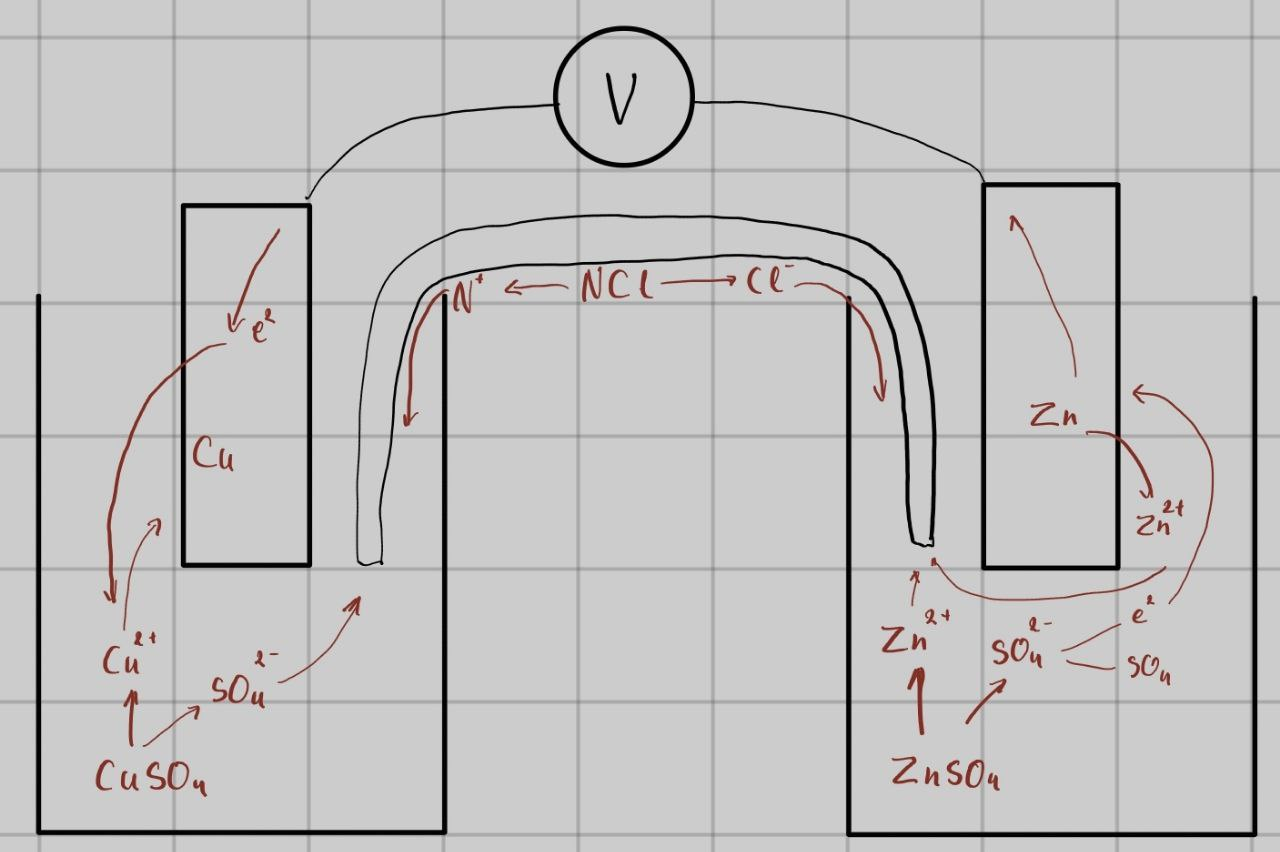
\includegraphics[width=1\linewidth]{Ex_1/s.jpg}
     \caption{Схема гальвонического элемента}
    \label{ex_1_1}
\end{figure}

Используя формулу Нерста: 

\begin{equation}
  E = E_0 - \cfrac{RT}{Fz}\ln\inner{\cfrac{a_{r}}{a_o}}  
\end{equation}

Примем $R = 8.81, \ F = 9.64\cdot10^4, T = 300^{\circ}F$

\begin{eqnarray}
  ZnSO_4 &\to& Zn^{2+} + SO_4^{2-} \\
  CuSO_4 &\to& Cu^{2+} + SO_4^{2-}
\end{eqnarray}

По таблице стандартный эл. потенциалов
 $E_{0Zn} = -0.763 V, \ E_{0Cu} = 0.337 V$.
  


 \begin{center}
     \begin{tabular}{l||l||l}
        & Elem. & $a_o/a_r$ \\
        1 & Cu & 1 \\
        1 & Zn & 1 \\
        2 & Cu & 0.1\\
        2 & Zn & 0.1\\   
        3 & Cu & 0.01\\   
        3 & Zn & 0.01\\   
      \end{tabular}
 \end{center}

\begin{equation}
  \varphi_1 = E_{Cu} - E_{Zn} = 0.337 + 0.763 = 1.1
\end{equation}

\begin{equation}
  \varphi_2 = E_{Cu} - E_{Zn} = 0.337 + 0.763 - \cancel{2}\cfrac{ 8.81 \cdot 3 \cdot \cancel{10^2}}{\cancel{2}\cdot9.64\cdot \cancelto{10^2}{10^4}}\ln\inner{0.1} = 1.04
\end{equation}

\begin{equation}
  \varphi_3 = E_{Cu} - E_{Zn} = 0.337 + 0.763 - \cancel{2}\cfrac{ 8.81 \cdot 3 \cdot \cancel{10^2}}{\cancel{2}\cdot9.64\cdot \cancelto{10^2}{10^4}}\ln\inner{0.01} = 0.97
\end{equation}

\begin{figure}[h]
  \centering
  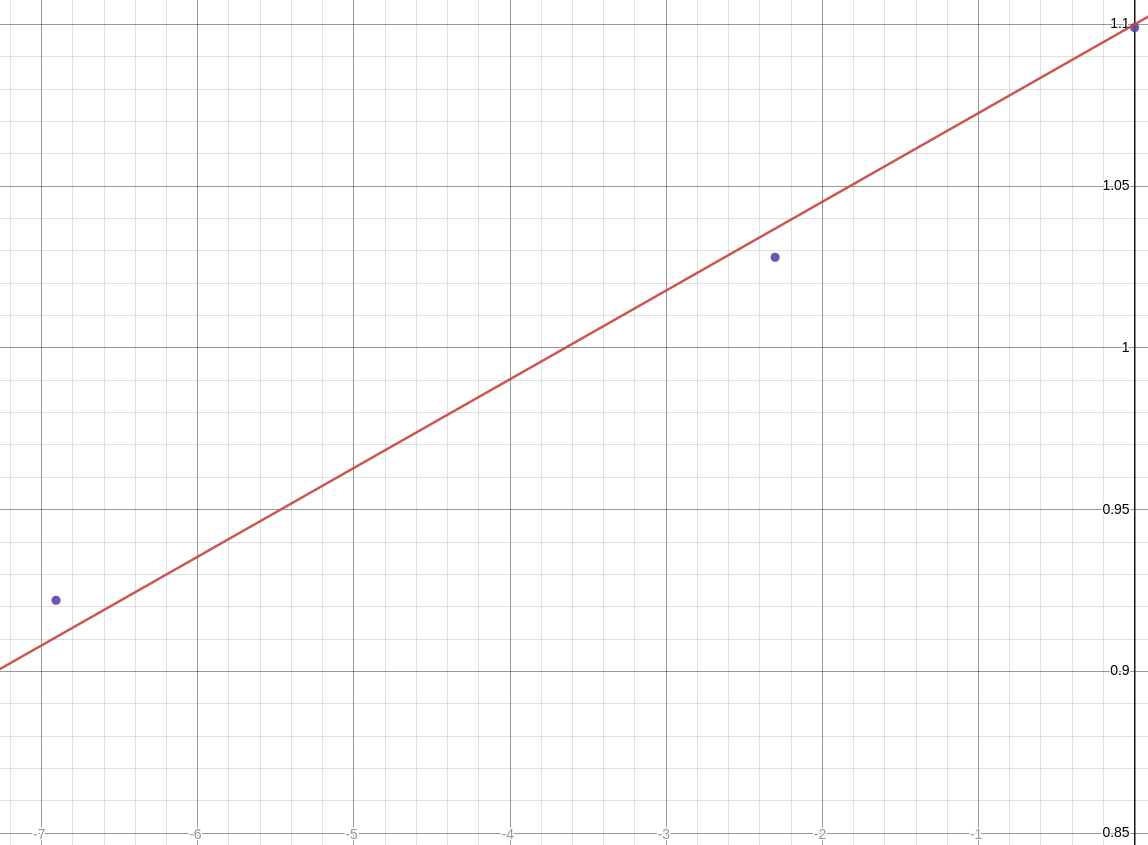
\includegraphics[width=1\linewidth]{Ex_1/plot.png}
   \caption{Схема гальвонического элемента}
  \label{ex_1_2}
\end{figure}





